% Chapter 1

\chapter{Physics of PENELOPE} % Main chapter title

\label{Chapter1} % For referencing the chapter elsewhere, use \ref{Chapter1} 

%----------------------------------------------------------------------------------------

% Define some commands to keep the formatting separated from the content 
\newcommand{\keyword}[1]{\textbf{#1}}
\newcommand{\tabhead}[1]{\textbf{#1}}
\newcommand{\code}[1]{\texttt{#1}}
\newcommand{\file}[1]{\texttt{\bfseries#1}}
\newcommand{\option}[1]{\texttt{\itshape#1}}

%----------------------------------------------------------------------------------------

%Outline for this section.
%Context: splice this section into the HEF paper as part of an extended
%methods section. Before talking about PENELOPE I need to state what it
%is that we need to model, and with what accuracy.
%1. Summarize what PENELOPE is.
%2. PENELOPE's treatment of elastic scattering and how it satisfies our requirements. How much detail can I omit here? For example, treatment of the 
%3. PENELOPE's treatment of inelastic scattering, including the Liljequist GOS model, and how it satisfies our requirements. 
%4. PENELOPE's treatment of the material-dependent energy-loss function.
%Discuss the program MATERIAL and justify penelope's use of Bragg's rule.
%May need to discuss the estar database?
% TODO: compare to the version of Dec 30 2016 (some changes were lost).
In this thesis I introduce the development of new techniques for the production of materials in the warm dense matter (WDM) regime, and for interrogation of the strucure and thermodynamic state of such systems using x-ray diffraction and (to a lesser extent) spectroscopy. The main developments include a scheme for single-shot determination of the static structure factors of WDM systems generated at laser plasma facilities; a new techinique for enhancing the density of deposited energy in WDM generated at fourth-generation X-ray sources such as the Linac Coherent Light Source (LCLS); and experimental results from an LCLS experiment that puts new constraints on the thermalization (both electronic and lattice) of a solid state material upon fs-scale XFEL heating. In addition to this WDM-focused research I discuss some secondary work on the development of software and electronics for energy- and position-sensitive pixel detectors including current applications in the context of soft x-ray laboratory and possible future ones in XFEL, synchrotron, and laser plasma facility-based experiments.

Before proceeding it is useful to define WDM in terms of the microphysical context it occupies. Fig. (which figure) presents a map of thermodynamic parameter space, with the logarithm of density and temperature on the horizontal and vertical axes, respectively. A few bounding curves can be identified. First, ionization occurs at temperatures exceeding approximately 1 eV; this is denoted by curve (a), which forms a boundary between the plasma and condensed matter regimes. Second, curve (b) indicates the boundary at which the Fermi energy is approximately equal to the average thermal energy $k_BT$; i.e. where the electron degeneracy parameter, $E_f/k_B T$ is of order unity. Third, curve (c) corresponds to a value of 1 for the ratio of the Coulomb energy to the thermal to the thermal one, also called the plasma coupling parameter  $\Gamma$. 

Above curves (a), (b) and (c) is the regime of classical plasma physics where, as a result of the weak interaction between neighboring ions ($\Gamma << 1$), collective interactions predominate over binary collisions and quantum statistics can be neglected ($\Lambda << 1$) except for the purpose of calculating blackbody spectra. In this regime continuous, classical modeling treatments are widely-used and fully validated (cites). Below curves (a), (b), and (c) is the low-temperature, intermediate-density realm of condensed matter physics, where the established theoretical framework is that of many-body quantum mechanics, wherein the potential landscape is built on the interaction between electrons and ion cores. In this framework finite-temperature effects are incorporated perturbatively. WDM occupies the transitional regime above curve (a) and near the intersection of curves (b) and (c), characterized by partial degeneracy and strong ion-ion coupling ($\Gamma$ and $\Lambda$ of order unity). As a result, treatments of plasma physics originating in the classical regime are not applicable to WDM. Solid state physics models similarly fail in the WDM regime due to large, non-perturbative effects of finite temperature on the structure and thermodynamics of WDM (cites).  

Modeling of the ionization potential depression (IPD) in a plasma is a case in point of the difficulties that manifest themselves with theoretical treatments of WDM. Adequate descriptions of IPD are given the Debye-Hueckel approximation and ion sphere model, which cover opposite regimes of high temperature and low density, and low density and high temperature, respectively. We here briefly introduce both model, with focus on the assumptions and approximations that they adopt.

The Debye-Hueckel model applies to a weakly-coupled plasma in local thermal equilibrium. It identifies the Poisson equation with the mean field generated by a population of Maxwell-Boltzmann-distributed ions or electrolytes. This results in the Poisson-Boltzmann equation which, when solved, gives the electrostatic potential produced by an arbitrary charge distribution. The condition for validity of the Debye-Hueckel model is for the Thomas-Fermi screening length (also called the Debye length) to be much larger than the mean inter-ion separation. This condition is satisfied at comparable temperatures, but lower densities, than those encompassed by the WDM regime. (check that this is right, and cite)
%Debye-Hueckel validity: cite 
%Electronic energy-levels in dense plasmas
%Richard M More
%Journal of quantitative spectroscopy & radiative transfer , 1982, Vol.27(3), p.345-357
% Need cites showing experimental validity of DH model

In the opposite limit, the ion-sphere model describes IPD in a low-temperature, high-density material (in this context IPD is more commonly referred to as pressure ionization). The picture offered by the ion-sphere model is that of a plasma with highly-correlated ion positions and therefore no close encounters between ion pairs. Each ion is treated as a sphere whose potential is unaffected by the presence of neighboring ions. (cite Stewart-Pyatt). The sphere radius is $R_0 = (3/4 \pi N_i)^{1/3}$, where $N_i$ is ion number density, while the orbital radius of the ion sphere's $n$th principal energy level is approximately $r_n = (n^2/Z_n)(0.529 \Angstrom$. For the $n$th bound state to exist it is necessary that $r_n \lte R_0$; thus, IPD manifests itself as a reduction in the number of bound states as a function of the inter-ion distance $R_0$.
% TODO: need stuff here on the validity of the ion sphere model
% Cite Zimmerman and More 1979

Constructing a model of ionization potential depression that is applicable in a high-density and disordered plasma is challenging because it requires abandoning all simplifying approximations invoked by the ion-sphere and Debye-Huekel models. (list the assumptions?) One manifestation of the community's uncertainty of the correct approach is the existence of two mutually-contradictory models for IPD, those of Stewart and Pyatt (cite) and Ecker and Kroll (cite). Though the Stewart-Pyatt model is more widely used and has the virtue of reproducing the ion-sphere and Debye-Hueckel behaviors in its limits (cite Crowley review article), its validity has been called into question by recent direct XFEL-measurements of IPD in Al heated to 180 eV (cite Ciricosta paper). More text here ............... Dig up key west talk........... Borrow language from physics 511 term paper....
% TODO: insert Fig. 2 from Ciricosta paper.
% TODO: talk about XRTS data interpretation issues


\section{Motivations for study of WDM}
In addition to the basic science questions intrisic to the WDM regime, there are a number of points of contact between WDM and other fields that have in recent years bolstered interest in it. We introduce a few here. Rework this.........

\subsection{Planetary Astrophysics}
The advent of laboratory systems capable of producing conditions approaching those of astrophysical systems has in recent years led to increasing overlap of research efforts in the astrophysics and high energy density physics communities. This integration has led to growth of experimental astrophysics as a subfield in its own right. Concommitantly, advances in computational power have brought many previously-inctractable physical regimes into the scope of numerical simulation.

The properties of dense, Fermi-degenerate plasmas at ~1 eV have direct relevance to the physics of planetary interiors. Examples include the equation of state of iron under conditions of the earth's core (pressure = 3 Mbar; T = 6000 K), which has consequences for the formation of earth's magnetic field. Similarly, modeling of the evolution and structure of gas giant planets depends on understanding of the equation of state of H under the regime of gas giant interiors. The existence of metallic H caused by pressure ionization at Mbar-scale pressures has been experimentally demonstrated; the presence of an accompanying first-order dielectric-to-metal transition has been postulated but is subject to substantial uncertaintly, due to the aforementioned limitations of current theory. Furthermore, the two-component phase diagrams of H with other species found in rocky planetary bodies have direct consequences not only on the structure of structure of gas giants, but also on their likely formation processes (i.e., planetary nebula gravitational collapse vs. planetesimal accretion) (cite Wilson MgO solubility paper). 
% cite Weir et al., Metallization of Fluid Molecular Hydrogen at 140 GPa
% cite Ebeling and Richert, PLASMA PHASE TRANSITION IN HYDROGEN 
and that of H at the temperature and pressure regime of gas giant planet interiors. 
%(cite koenig et al, doi: http://dx.doi.org/10.1088/0741-3335/47/12B/S31)

Another case in which the material properties of warm dense matter determine the behavior of an astrophysical object is that of white dwarves, whose envelopes consist of a hot, partially Fermi-degenerate plasma. Modeling the cooling of white dwarves is a topic of interest (cites), especially in the context of the importance of type 1a supernovas as `standard candles' for measuring distances to distant galaxies. Doing so, however, requires knowledge of stellar envelope's opacity, equation of state, and transport properties, many of which are currently unknown to within factors of order unity. The absence of understanding of even the simplest available system--the hydrogenic one-component plasma--underscores the problem's difficulty. 
% cites needed, see pg 58 of x-games




PENELOPE performs Monte Carlo simulations of coupled electron-photon transport in arbitrary materials in the energy range of 100 eV to 1 GeV. It uses a mixed simulation method that treats soft interactions (that is, those involving small angular deflections) with a multiple-scattering approach while individually simulating hard interactions. It is paired with a geometry-definition program, PENGEOM, that allows defining samples with volumes of different material composition separated by arbitrary quartic surfaces.


\section{Types of interactions}
In this section we consider the interactions that must be simulated to accurately model the spatials distribution of energy in a nanostructured target material heated by x-ray photons with energy on the order of 10 keV.
PENELOPE simulates the following interactions: electron scattering (elastic and inelastic), Bremsstrahlung emission, photon scattering (both elastic (Rayleigh) and inelastic (Computon)), photoelectric absorption and Auger emission, x-ray fluorescence, and pair production and anihillation. 
Figs. \ref{fig:sp} and \ref{fig:photon_sigma} show the energy dependence of the relative strengths of the above electron and photon interactions, respectively. 
Several of the processes have negligible or nonexistent roles on the < 10 keV energy scale considered in the current work, allowing us to limit our scope to the electron scattering and photoabsorption (with consequent fluorescence and Auger emission).

\begin{figure}[h] \label{fig:col_rad}
\caption{Collisional and radiative electron stopping powers as a function of energy (cite)}
\centering
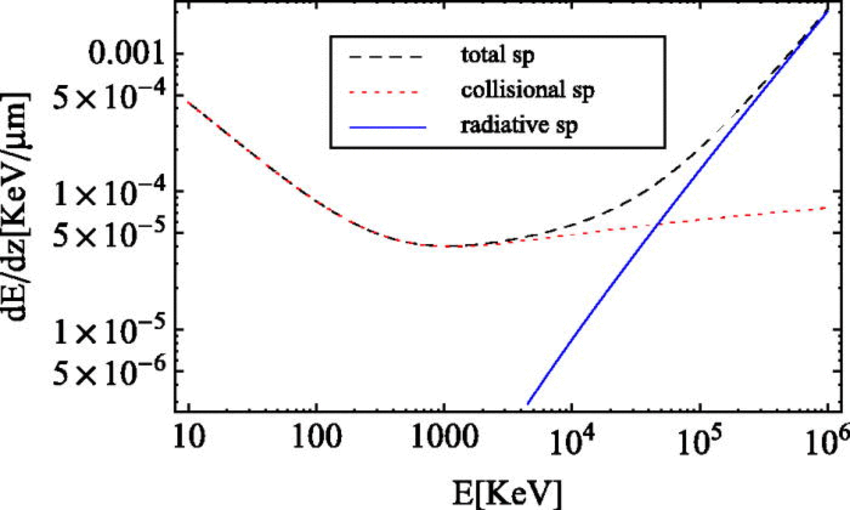
\includegraphics[scale=0.4]{../Figures/collisional_sp.png}
\label{fig:sp}
\end{figure}

\begin{figure}[h] 
\caption{Photon cross section components in C as a function of energy (cite LCL and Hubbell 1980)}
\centering
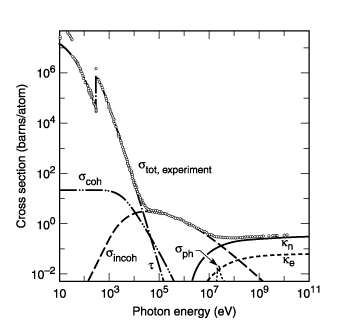
\includegraphics[scale=1]{../Figures/photon_sigma.png}
\label{photon_sigma}
\end{figure}

In what follows we introduce the physics of photoabsorption and elastic and inelastic scattering with attention to each process's contribution to the spatial distribution of deposited energy in a relaxation cascade beginning with photoionization by a hard x-ray photon. We discuss standard modeling approaches relevant to the 100 eV-10 keV regime, in addition to cursory overviews of PENELOPE's treatments within the limited scope relevant to the current regime of interest. % (including, for example, including relativistic energies).
%In the case of inelastic electron scattering, where numerous treatments of the central quantity (the generalized oscillator strength, or GOS) exist, we discuss necessary common features of all GOS models before introducing PENELOPE's specific treatment.

\subsection{Fluorescence}
Fig (insert fig. 2.2 from penelope manual) illustrates the photoionization of inner atomic shells and introduces the notation used to describe atomic energy leves and transitions between them.
Both the photoelectric effect and secondary (Auger) emission resulting from high-energy atomic excitations can be accurately modeled using established treatments that combine theoretical calculation of atomic states via self-consistent modeling (cite Pratt et al. 1973) with experimental data. Associated quantities are compiled in databases; PENELOPE uses tabulated ionization energies from Carlson (cite Carlson et al.) and photoelectic cross sections from the LLNL Evaluated Photon Data Library (EPDL). The EPDL additionally provides emission probabilities for fluorescence photons and Auger electrons in the relaxation of ionized atoms to the ground state.

\begin{figure}[h] 
\caption{Atomic energy levels of the first three principal quantum numbers (left) and corresponding allowed radiative transitions (right).}
\centering
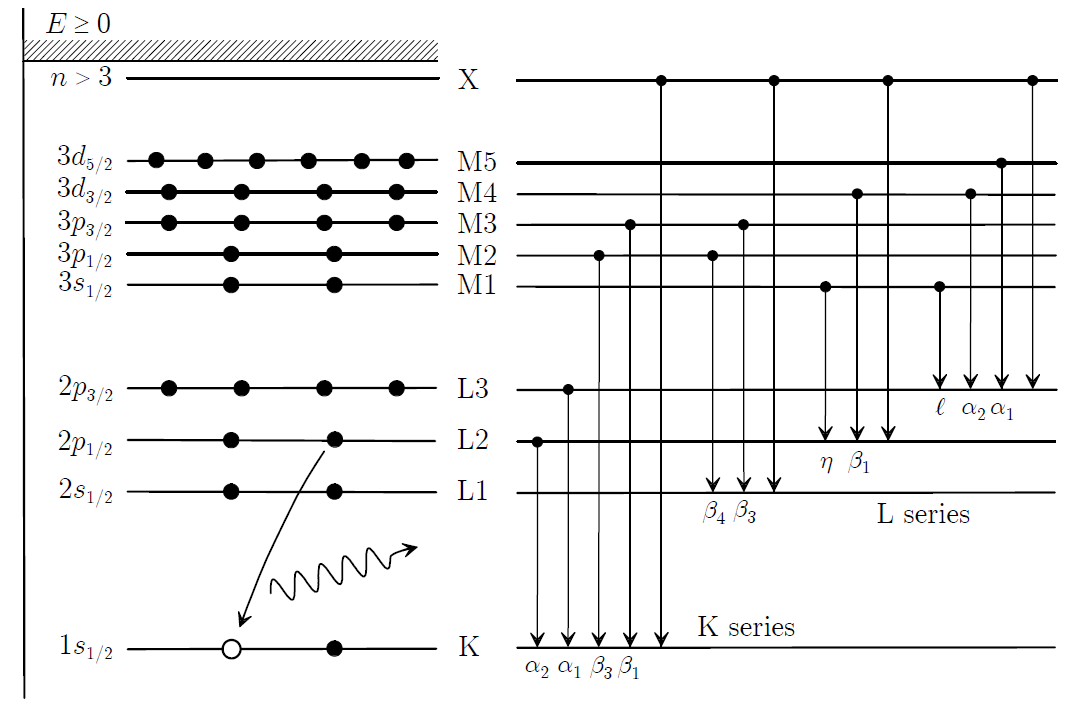
\includegraphics[scale=0.4]{../Figures/penelope_2_2.png}
\label{fig:photoionization}
\end{figure}



\subsubsection{Assumptions}
The above data sources are known to be accurate to the $1\%$ level above $1$ keV, under the condition (assumed by PENELOPE) of low incident photon densities, such that only single-electron transitions occur (cite PENELOPE manual).

PENELOPE assumes that incident photons are unpolarized and consequently fails to reproduce the polarization-dependent angular distribution (cite?) of emitted electrons. 
We note that it does incorporate the angular distribution from Sauter's (cite sauter 1931) treatment of relativistic photoelectron emission--which, however, reduces to isotropic emission in the nonrelativistic regime covered here.



\subsection{Elastic scattering}
Elastic scattering of electrons refers to interactions that do not alter target atoms' states. 
% TODO: consider moving some of the below text to the end of this section
%PENELOPE uses the static field approximation (cite Mott and Massey), which is accurate above energies of a few hundred eV (cite PENELOPE manual, page 102) but introduces a considerable error to the elastic DCS at and below 1 keV (discuss in next section). 
%An atom's electrostatic potential is expressed in terms of the nuclear and electronic charge densities, $\rho _n (r)$ and $\rho _e (r)$ respectively: 
%
%% TODO: nuclear charge should be a point
%\begin{multline}
%\phi (r) = e~4~\pi [\frac{1}{r}\int_0^{r}\rho(r')r'^{2} + \int_r^{\infty}\rho_n(r')r'dr'] -\\ e~4~\pi \frac{1}{r} \int_0^r\rho_e(r')r'^2 dr' + \int_r^\infty \rho_e(r') r' dr'].
%\end{multline}
%We note that, although PENELOPE accounts for the effect of the finite nuclear size on the elastic DCS, we simply treat the nucleus as a point source as this is sufficient for electrons with energy below 1 MeV. (cite PENELOPE manual)

%Fermi distribution:
%
%\begin{equation}
%\rho_n(r) = \frac{\rho_0}{exp[(r - R_n)(4ln3/t)] + 1},
%\end{equation},

%(cite Hahn et al. 1956 and understand the orgin of this expression)  $R_n$ is the mean radius and $t$ is the 'skin` thickness of $\rho_n$ defined in Hahn et al. 1956. 

%The total interaction energy for electrons is
%
%\begin{equation}
%V(r) = -e\phi(r) + V_{ex}(r),
%\end{equation}
%
%where $V_{ex}(r)$ is a local approximation of the exchange interaction between the incident electron and atomic electrons. The angular distribution of elastic scattering off this central field is axially symmetric, and the DCS $d\sigma_{el}/d\Omega$ may therefore be expanded into a sum of Legendre polynomials. [Citing Salvat 2005 or Walker, describe how the phase shifts are obtained from the Dirac radial wave functions. What's the role of the exchange term in all this?]

%\section{First view: Yukawa potential}
The simplest widely-used model for elastic scattering of electrons in a solid is the semi-classical approach of Wentzel and Lenz (Egerton page 114 ), known as the Lenz model, which uses the Yukawa potential for the interaction between a fast electron and a target atom:

\begin{equation}
	V(r) = \alpha^2 \frac{e^{-r/r_0}}{r}
\end{equation}

%sufficient to derive the approximate differential cross section of elastic scattering and to describe its influence on the spatial distribution of scattered electrons at our energy scale of interest. 

The first Born approximation gives the amplitude for a particle's scattering off of a spherically symmetric potential as
% TODO cite http://itp.uni-frankfurt.de/~valenti/SS14/QMII_2014_chap1.pdf or other

\begin{equation}
	f(\theta) \simeq -2 \frac{m}{\hbar^2 q} \int_0^\infty r V(r) \sin (qr) dr
\end{equation}

Substituting (how do I reference equations) into (), yields 
%from http://itp.uni-frankfurt.de/~valenti/SS14/QMII_2014_chap1.pdf
%TODO: make the notation here consistent.
\begin{equation}
	f(\theta) \simeq -2 \frac{m \alpha^2}{\hbar^2 q} \int_0^\infty e^{-r/r_0} \sin (qr) dr = -\frac{2m\alpha^2}{\hbar^2 (r_0^{-2} + q^2)},
\end{equation}

therefore giving the following differential scattering cross section:
$$
\frac{d\sigma}{d\Omega} = |f(\theta)| = \frac{4 Z^2}{a_0^2 k_0^4} \frac{1}{(\theta^2 + \theta_0^2)^2},
$$
where $k_0 = m_0 v$ is the momentum of the incident electron, $\theta_0 = (k_0 r_0)^{-1}$ is the characteristic angle for elastic scattering and $a_0 = 4 \pi \epsilon_0 \hbar^2/m_0 e^2$ is the Bohr radius.

Using the Thomas-Fermi model, Wentzel and Lenz obtain $r_0 = a_0 Z^{-1/3}$ (cites). Doing this substitution and integrating over scattering angles gives
\begin{equation}
\sigma_e = \int_0^\pi \frac{d\sigma}{d\Omega} 2 \pi sin \theta d \theta = \frac{4 \pi}{k_0^2} Z^{4/3}
\end{equation}

% TODO: copper->iron
We thus see that the angular deflections produced by elastic scattering decrease with increasing energy. For 10 keV electrons $\theta_0 \simeq 0.1$ rad and $\sigma_e = 4.2 \times 10^{-20}~\mathrm{m}^2$. The elastic mean free path, an alternate measure of the collision frequency, is equal to $\lambda_e = 1/(\sigma_e n)$, where $n$ is atomic number density. As an example, inserting the value of $n$ for Fe yields 2.8 \AA (at the same 10 keV electron energy) (\emph{sounds far too small; check this calculation}). This corresponds to a large number of collisions on length scales of interest (> 10 nm) which, combined with the appreciable value of the characteristic scattering angle, demonstrates that elastic scattering has a substantial influence on the propagation of electrons below 10 keV. 

Taking the atomic number of density of Fe, the mean free path between inelastic collisions is (insert the right expression) = (insert the right number). The corresponding expectation value of angular deflection per distance traveled is (insert the right number). In comparison, the inelastic mean free path of 10 keV photons in Fe (potential see-saw here is (insert number). where should i introduce inelastic scattering?) This suggests that path deflections caused by elastic scattering will have a significant influence on the spatial distribution of energy deposited 10 keV-scale electrons in Fe and other mid-Z materials. 

Despite its simplicity, the Lenz model gives total cross sections to within 10 \% for light elements (cite Geiger 1964). For heavier species it underestimates the small-angle differential cross section (Fig. \ref{fig:e3.3}) but correctly reproduces the large-angle DCS.

\begin{figure}[h] 
	\caption{Angular dependence of elastic DCS of 30 keV electrons from a Hg atom under the Lenz model using the Wentzel potential (solid), and based on Hartree-Fock (dotted), Hartree-Slater (dot-dashed) and Dirac-Slater (dashed) wavefunctions.  \parencite{Reference1} }
\centering
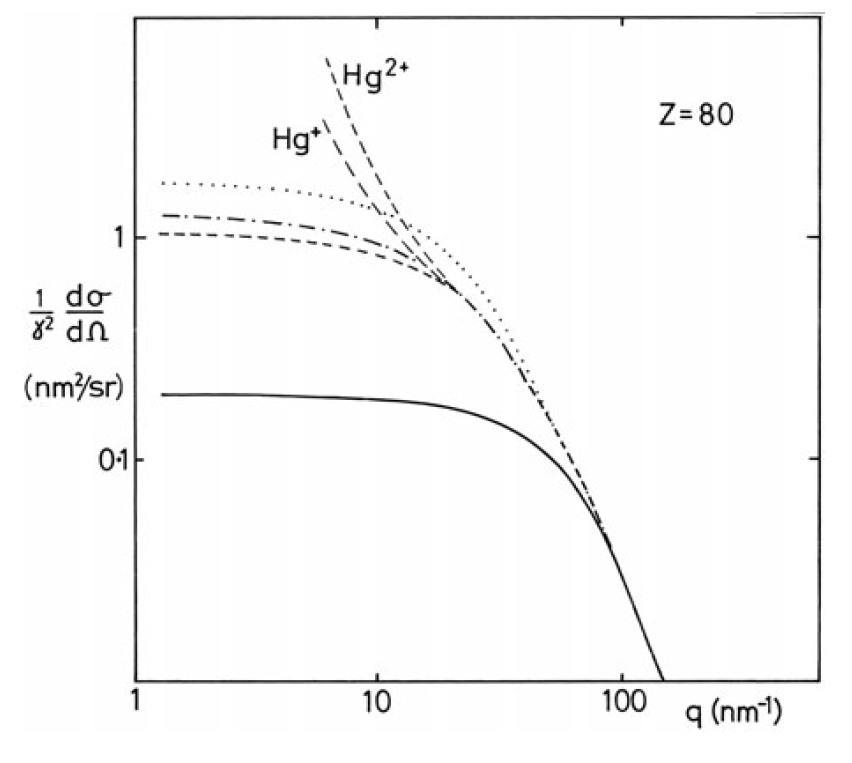
\includegraphics[scale=0.5]{../Figures/egerton_3_3.png}
\label{fig:e3.3}
\end{figure}

More accurate approaches use iterative (e.g. Hartree-Fock) solutions to the Schroedinger equation (or of the Dirac equation, where relativistic and spin effects are needed) to solve for the atomic potential. (cite rez 1984 or starostin, applicability of the born approximation to collisions between electrons and excited atoms). Additionally, partial wave approaches can be used to avoid the Born approximation in regimes for which it fails (low electron energy and high-Z species). PENELOPE combines the above techniques: it solves the partial-wave expanded Dirac equation with a potential based on the Dirac-Fock electron density of Desclaux (1975, see citation on pg 102 of penelope manual) and exchange interaction of Furness and McCarthy (1973). We will elaborate on PENELOPE's modeling of elastic scattering only within the narrow concern of assesing its range of applicability; for more detail the reader may refer to chapter 3 of the PENELOPE manual. 


% Fig. (fig reference) shows the angular dependence of scattering for Fe. 

\section{Inelastic scattering}
Inelastic collisions are the dominant mechanism for energy loss of electrons up to above 10 keV (\ref{fig:col_rad}).
%The double differential cross section for collisions with momentum transfer $q$ and energy loss $\omega$ is given by Fano (cite Fano 1963, see page 114 of PENELOPE manual) as

In an atomic system, the differential cross section for a transition from initial state wavefunction $\psi_0$ to final state wavefunction $\psi_n$ is

\begin{equation} \label{bornDCS}
\frac{d\sigma_n}{d\Omega} = \frac{m_0}{2\pi \hbar^2}^2 \frac{k_1}{k_0} \mid \int V(r) \psi_0 \psi_n exp(i q r) d\tau \mid ^2
\end{equation}
%TODO: fix the notation here. How does one do bolded text? dot products?
where $\textbf{k}_0$ and $\textbf{k}_1$ are the wave vectors of the incident electron before and after scattering and $q = \hbar (\textbf{k}_1 - \textbf{k}_1)$ is the corresponding momentum transfer. 

At nonrelativistic velocities the potential between electron and atom may be expressed as the following sum of Coulomb potentials of the nucleus and atomic electrons:

\begin{equation} \label{cpotential}
V(r) = \frac{Ze^2}{4\pi \epsilon_0 r} - \frac{1}{4 \pi \epsilon_0} \sum_{j = 1}^Z \frac{e^2}{\mid \mathbf{r} - \mathbf{r_j} \mid}
\end{equation}
%TODO
%(define whichever quantities haven't been introduced yet)
Substituting the second term of equation \ref{cpotential} into \ref{bornDCS}, we note that the nuclear potential is independent of the coordinates of the atomic electrons and can therefore be removed from the integral. The orthogonality of the wave functions $\psi_n$ implies that the nuclear potential does not contribute to inelastic scattering; the expression for the differential cross section of inelastic scattering is therefore:

\begin{equation} \label{inelasticDCS}
\frac{d\sigma_n}{d\Omega} = (\frac{4}{a_0^2 q^4}) \frac{k1}{k0} \mid \epsilon(q)\mid^2,
\end{equation}

where

\begin{equation}
	\epsilon_n = \int \psi_n \sum_j e^{i q r_j} \psi_0 d\tau.
\end{equation}


The generalized oscillator strength is an important related quantity:

\begin{equation}
f_n(q) = \frac{E_n}{R} \frac{\mid \epsilon_n(q)\mid ^2}{(q a_0)^2},
\end{equation}


where $R = (m_0 e^4 / 2)(4 \pi \epsilon_0 \hbar)^{-2}$, the Rydberg energy, and $E_n$ is the energy change of the transition. 

The GOS is in general continuous and therefore better expressed as a density with dimensions 1/energy, i.e. $df(q, E)/dE$. This allows us to write the double-differential cross section of inelastic scattering:

\begin{equation} \label{inelastic_DDCS}
\frac{d^2\sigma}{d\Omega dE} = {4 R}{Eq^2} \frac{k_1}{k_0} \frac{df}{dE}(q, E),
\end{equation}

TODO: calculate a typical inelastic scattering cross section for comparison elastic scattering. The fact that the ratio is of order unity demonstrates that both matter.

\subsection{Dielectric function}
While this formulation makes it possible to calculate the GOS and associated quantities starting from an atomic model, in solid state systems the scattering cross section of outer-shell bonding is influenced by collective effects and chemical bonding. It's therefore preferable to describe the inelastic scattering of an electron off a solid using the solid's dielectric response function, $\epsilon(q, E)$. 

Ritchie (cite Ritche 1957) showed, using Poisson's equation and fourier transforms, that an electron moving in the z-direction in an infinite medium experiences a force of the following magnitude opposite its direction of motion: 


\begin{equation} \label{stp}
\frac{dE}{dz} = \frac{2\hbar^2}{\pi a_0 m_0 v^2} \int \int \frac{q_y \omega Im[-1/\epsilon(q, \omega)]}{q_y^2 + (\omega/v)^2},
\end{equation}

% TODO: vectors?
where $q_y$ is the component of the momentum transfer vector perpendicular to $v$ and $\omega = E/\hbar$ is an angular frequency. This quantity is referred to as the stopping power. It can be expressed in terms of the previously-defined DDCS:

\begin{equation} \label{stp2}
\frac{dE}{dz} = \int \int n E \frac{d^2\sigma}{d\Omega dE} d\Omega dE,
\end{equation}

%\frac{d^2\sigma}{d\Omega dE} = 

where $E$ is energy loss and $\Omega$ is solid angle. By equating equations \ref{stp} and \ref{stp2} in the small-angle limit it can be shown, by comparison with the atomic treatment (cite), that 

$$
\frac{df}{dE}(q, E) = \frac{2E}{\pi E_a^2} Im[\frac{-1}{\epsilon(q, E)}],
$$

thus demonstrating the equivalence of the atomic and dielectric approaches.

Note, finally, that the GOS fully determines the the value of equation \ref{inelastic_DDCS} within the first Born approximation. As such, given the potential of equation \ref{bornDCS} all modeling of the inelastic scattering of electrons at intermediate energies (1 keV - 300 keV) reduces to construction of a GOS model. 


%For a continuous energy loss spectrum, it takes the differential form $dF/dE(q, E)$, a density with respect to energy loss.

% TODO: move this somewhere
% We note that PENELOPE incorporates Fano's (1963) relativistic treatment of inelastic scattering of electrons in condensed media in place of the current treatment. 

\subsection{Modeling the generalized oscillator strength}
Analytical expressions for the GOS are known for only two simple cases of the free electron gas and hydrogen atom. In practice, however, it has been shown that the physics of inelastic scattering is mostly determined by a few global features of the GOS (cite Salvat and Fernandez-Varea, 1992) and that relatively simple models are therefore adequate in most situations.


% TODO: read Salvat and Varea, 1992
The GOS is conventionally represented as a two-dimensional surface plot called the Bethe surface (Fig. \ref{fig:bethe}). 
We identify two constraints on the behavior of the Bethe surface which any GOS model must reproduce. First, in the limit $Q\rightarrow 0$, the GOS of the dielectric formulation becomes proportional to  the optical oscillator strength $Im[-1/\epsilon(0, E)$, which is experimentally constrained by x-ray emission measurements. Second, in the limit of large momentum transfer the most probable energy loss is equal to the kinematically-determined value for collision between two free electrons, $E = q^2/2$. (cite Sorini). The corresponding trace in energy and momentum is a feature of the Bethe surface known as the Bethe ridge.

\begin{figure}[h] 
\caption{Bethe surface for ionization of the K shell in C.......... (cite)}
\centering
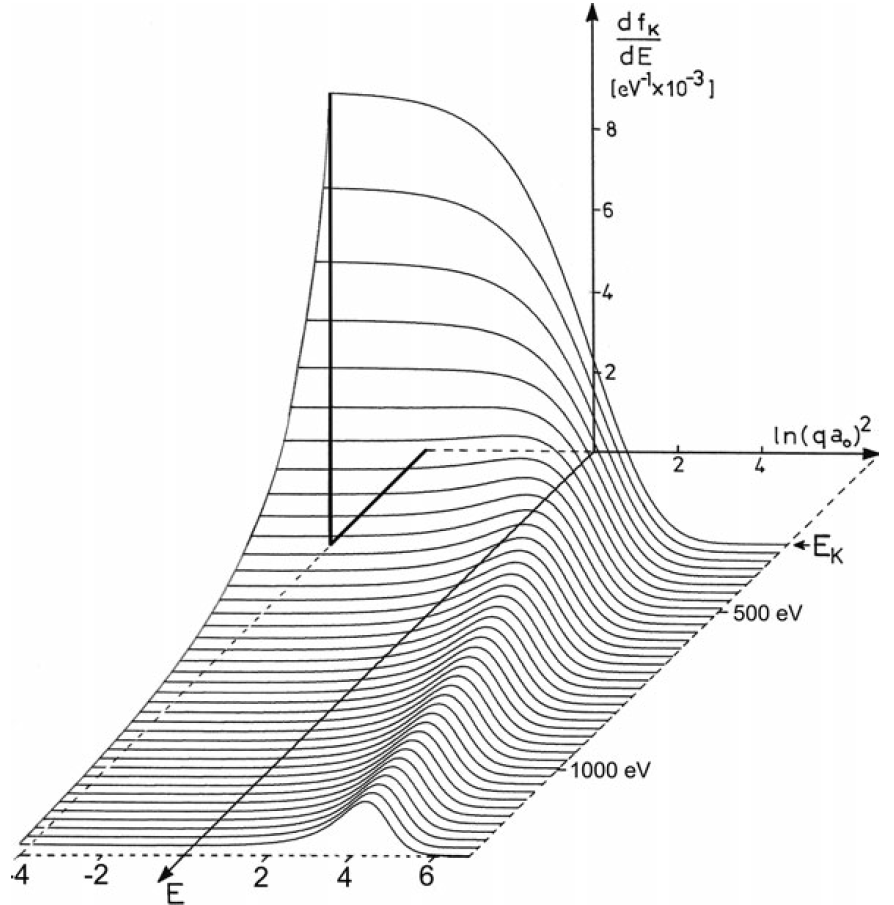
\includegraphics[scale=0.5]{../Figures/bethe.png}
\label{fig:bethe}
\end{figure}

As in Compton scattering, the shape of cuts throught the Bethe surface (i.e. spectra of scattered intensity as a function of energy at fixed momentum transfer) is determined by the momentum distribution of atomic electrons. Certain models, such as that of Sorini et al (cite sorini 2006), derive a value for the width of the Bethe ridge from Fermi velocity calculations. PENELOPE adopts a simpler form based on the `$\delta$ -oscillator' model of Liljequist (cite Liljequist 1983) which splits the GOS into contributions from generalized `shells' (each corresponding to either an atomic shell or a collective excitation). The total GOS under this model is a sum over indices \emph{k} of the shells:

$$
\frac{df(q, E)}{dE} = \Sigma f_k [\delta(E - E_k) \Theta (q_k - q) + \delta(E-q) \Theta(q - q_k)],
$$
where for the \emph{k}th shell $f_k$ is the shell's number of electrons, $q_k$ is the cutoff recoil energy, and $E_k$ is the shell's resonance energy. $Q_k$ is equal to the shell's binding energy $U_k$ (excluding the band, for which it is set to 0), and $E_k$ is computed from from $U_k$ and the material's mean electron density, following Sternheimer (cite Sternheimer 1952). Within this model the GOS is fully determined by the shells' occupations and cutoff (binding) energies $U_k$, which PENELOPE obtains from Carlson (cite Carlson 1975). It is possible, optionally, to direct PENELOPE to fit its GOS model to experimental stopping power data provided in material input files. It performs this fit through reweighting of the GOS model's oscillators (\emph{this is actually a guess, as the PENELOPE manual is totally opaque about how the GOS/DDCS is fit to stopping power input data. Better understanding would require me to revisit PENELOPE's code or contact the authors}).

Substantial additional detail on the construction and interpretation of PENELOPE's GOS model can be found in its manual.

% TODO: talk about convergence with the Bethe model
% readily measured experimentally via the photoelectric cross sections in the diplole limit. (TODO: show this relationship between the photoelectric cross section and GOS mathematically, or cite Fernandez-Varea 1993 a). (cites. also, is this true (about the zero-angle energy loss spectrum?). Where Q is much larger than binding energies of the target electrons, the latter behave as though they were free and the GOS is described by the Bethe ridge, a peak along $W = Q$. 

% TODO numerical implementation and coarse graining
% TODO fluorescence
\section{Accuracy and useful regimes}
In the context of simulation of nanostructured materials, errors in PENELOPE's DCSs for electron scattering originate from both (1) the limited range of validity of PENELOPE's physical models with respect to the bulk properties PENELOPE seeks to reproduce, and (2) from the difference between scattering DCSs of ambient-condition bulk materials on the one hand and high-temperature nanostructured materials on the other. We address these two issues in combination.

As mentioned previously, a material's inelastic scattering DCS is fully determined by its loss function, the imaginary component of the dielectric function. Any difference between the responses of bulk and nanophases arises from the contribution to the loss function of collective electronic excitations, i.e. plasmons. Plasmon modes in nanostructured materials form a large research topic on their own (find and cite review article on surface plasmons in nano-materials), but there there has been little (no?) (cites) prior work in the context of high-temperature dense matter. The study of heated nanophase materials thus manifests itself as both a problem and an opportunity. On the one hand, the lack of experimental data and accurate modeling makes it impossible to fully quantify the inaccuracy of simulations of ambient, bulk materials. On the other hand, XFEL heating experiments could be used to discriminate between computed dielectric response functions and their underlying finite-temperature electronic strucure theory--to the extent that alternative models generate experimentally measureable differences in inelastic DDCSs. We thus suggest that XFEL heating of nanostrucured materials could enable a joint modeling/experimental program to validate WDM electronic structure theory.

\subsection{Low-energy loss DCS} \label{ledcs}
In the current situation, wherein the plasmon contribution to the loss function is not known, we can take advantage of the fact that plasmon resonance are confined to energy losses smaller than approximately 100 eV. The influence of the low-energy region of the loss function on the spatial distribution of deposited energy can therefore be bounded using the continuous slowing down approximation (CSDA) of 100 eV electrons. The CSDA for electrons of energy $E_0$ is the following integral over stopping power: 

$$
l_{CSDA} = \int_{E_{final}} ^ {E_0} (\frac{dE}{dz})^{-1},
$$

where $E_{final}$, the final energy of the electron, is usually taken to be 10 eV. For elements heavier than boron, $l_{CSDA} < 10$ nm for $E = 100 eV$. We therefore conclude that inaccuracy in treatments of collective excitations affect the spatial distribution of energy deposited by electrons on a length scale below 10 nm (Fig. \ref{fig:csda}) (\hyperref[cite]{http://xdb.lbl.gov/Section3/Sec\_3-2.html}) 

\begin{figure}[h] 
\caption{CSDA range as a function of energy for several materials, based on stopping powers of..... (cite)}
\centering
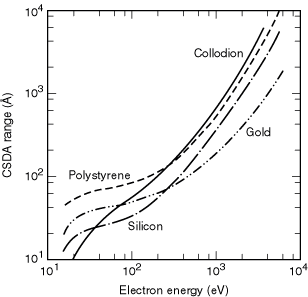
\includegraphics[scale=0.7]{../Figures/csda.png}
\label{fig:csda}
\end{figure}

\subsection{Energy cutoffs} \label{cutoffs}
PENELOPE stops simulation of an electron's motion once its energy drops below a prescribed cutoff value; at the endpoint of an electron's simulated track all of the electron's final energy is deposited at its final position. The resulting distortion in the spatial distribution of deposited energy can be bounded, as above, using the CSDA. PENELOPE's cutoff energy can be set as low as 50 eV. Assuming this value is chosen, the resulting error is much smaller than the bound from section \ref{ledcs} on the error attributed to inaccuracy in the low-energy dielectric function. Simulation error due to PENELOPE's energy cutoff can therefore be safely neglected.

% TODO: see berger and seltzer 1982 calculation of mean excitation energies
\subsection{Elastic scattering}
% TODO also need to talk about the absorption correction / dual channel thing
PENELOPE's use of the static field approximation in its elastic scattering model introduces a low-energy error in the DCS due to the effect of the polarizability of atomic charge (cite Salvat 2003). The size of this error is 20\% at 1 keV and 50\% at 100 eV (PENELOPE manual, pg. 102). The CSDA range at 1 keV, where uncertainty at the DCS level is considerabe, ranges from 10 nm for high-Z elements to over 100 nm for low-Z ones. Because the results of the PENELOPE simulations discussed in chapter (which chapter?) are sensitive to errors on the 10 nm - 100 nm length scale, the CSDA does not usefully constrain the elastic DCS model's contribution to uncertainty in the spatial distribution of deposited energy. 

A crude estimate taking into account the magnitude of uncertainty in the elasatic DCS may be obtained by considering elastic scattering of an electron as a correlated random walk. Given a mean free path $\lambda_e$ and characteristic scattering angle $\theta_0$, the number of steps after which the electron's direction of motion becomes uncorrelated with its initial direction is of the order $n = \pi/\theta_0 \lambda_e$. The number of elastic scattering events an electron experiences as it slows from an energy of 1 keV to 100 eV (the previously-established--but arbitrary--cutoff below which the treatment of section \ref{ledcs} applies) is

sketch: basically I have to calculate the number of scattering events, and associated dephasing of the electron's direction, for several `bins' of energy between 100 eV and 1 keV. For each bin we calculate the equivalent number of steps under an uncorrelated random walk. This yields an expected displacement proportional to the square root of the number of steps in the uncorrelated random walk, which we can multiply by the elastic DCS uncertainty in order to get an associated displacement uncertainty. All displacement uncertainties can then be added in quadrature, yielding a final uncertainty. 


\section{Inelastic scattering}
% TODO In the prior discussion of scattering models I need to add the equation for the inelastic/elastic scattering ratio and also compare characteristic scattering angles.
Inelastic scattering has much smaller characteristic angles than elastic scattering scattering but comparable total cross sections. As a result the influence of angular deflections by inelastic scattering on the propagation of electrons is relatively small. The effect of uncertainties in the inelastic scattering DDCS can thus be neglected, and we confine our attention to uncertainty at the level of the stopping power, a more coarse-grained quantity.

Fig \ref{fig:stp_accuracy} compares PENELOPE's computed stopping powers and inelastic mean free paths (for what???) to several experimental datasets. The level of disagreement between different datasets is of the order 2 in the 1 keV - 10 keV energy loss range; the discrepancy between PENELOPE's modeled stopping power and the experimental datasets is also of this order. Because all transport lengths are proportional to stopping power we must thus contend with a factor of 2 uncertainty in the length scale of computed spatial distributions--far larger than any of the other uncertainties we have considered until now. 

The conclusions of chapter (WHICH CHAPTER?) can nevertheless be conserved, with one modification, if we consider PENELOPE's error in modeling the 1 - 10 keV stopping power as an unknown constant-factor scaling in stopping power. Such an uncertainty corresponds to an unknown scaling of both (1) the length scale of spatial distributions of deposited energy and (2) the flux magnitude of nonlocally-transported energy crossing a given material interface. To give a simple illustration, consider a one-dimensional configuration consisting of an infinite extent of source material from $x = -\infty$ to $x = \infty$. When the sample receives x ray illumination of magnitude unity at position $x0$ the density distribution $\rho(x)$ of deposited energy is given by a response function $f(x)$ (fully determined by the sample material's stopping power and incident x-ray spectrum): $ \rho(x) = f(x - x0) $. If the material is uniformly illuminated by x rays in the region spanning $x = 0$ to $x = \infty$ then (in arbitrary units):

$$
\rho(x) = \int_0^{\infty} f(x - x') dx'.
$$

Under the substitution $f(x) \rightarrow g(x) = f(c x)$ (equivalent to scaling $dE/dz \rightarrow (1/c) dE/dz$ of the stopping power), and maintaining normalization of the response function, the distribution becomes:

% TODO: there's something wrong here
$$
\rho'(x) = \int_0^{\infty} c f((c (x -  x'))) dx = \int_{cx}^{\infty} f((u)) u.
$$

Therefore constant-factor scaling of the stopping power is equivalent to a change in units of length, implying that, under our assumed form of the uncertainty in $dE/dz$, and adding the assumption that the unkown scaling factor $c$ is equal for all materials, the simulated spatial distributions of deposited energy density are correct up to a uniform scaling of the sample geometry. 

%all the modeling error is captured by deviations in the stopping power.



\begin{figure}[h] 
\caption{Stopping power and inelastic mean free path for electrons as a function of energy in Al..... (cite)}
\centering
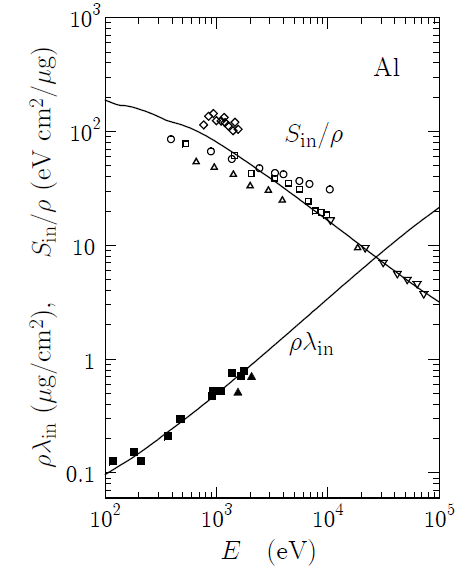
\includegraphics[scale=0.7]{../Figures/penelope_3_11.png}
\label{fig:stp_accuracy}
\end{figure}

\section{Dosimetry}
PENELOPE's dosimetry includes both linear energy transfer from radiation to matter and the contribution of particle track ends, as mentioned in section \ref{cutoffs}. At the energy scales of interest the former contribution may be neglected, and the distribution of energy deposited by a particle shower is entirely dependent on simulated inelastic scattering events. PENELOPE's dosimetry calculation is tied to the termination of electron tracks: when an electron's energy drops below the (previously-defined) cutoff value its simulation ceases, and its entire energy is deposited at the track's endpoint.  Similarly, the energy loss of soft inelastic collisions (ones having energy loss greater than the cutoff energy $W_{cc}$) is deposited locally (whereas hard inelastic collisions generate secondary electrons that are individually tracked). 

Coarse-graining of the dose distribution is done by dividing the simulation volume into a three-dimensional grid of cells, in each of which PENELOPE calculates the total dose of deposited energy. This grid is defined by the parameters GRIDX, GRIDY, GRIZ and GRIDBN in PENELOPE's input. 
% see section 5.2.1.2 in penelope manual

% TODO itemize with numbers

%TODO: Settle on one notation. E or W for energy loss?
%TODO: introduce the dielectric formulation of the ddcs?
%TODO: introduce the GOS in the first expression for the DDCS.


%NOTES:
%See appendix a in Egerton for justification of the simplified interaction potential for an incident electron and an atom below 300 keV. 


%\section{Welcome and Thank You}
%Welcome to this \LaTeX{} Thesis Template, a beautiful and easy to use template for writing a thesis using the \LaTeX{} typesetting system.
%
%If you are writing a thesis (or will be in the future) and its subject is technical or mathematical (though it doesn't have to be), then creating it in \LaTeX{} is highly recommended as a way to make sure you can just get down to the essential writing without having to worry over formatting or wasting time arguing with your word processor.
%
%\LaTeX{} is easily able to professionally typeset documents that run to hundreds or thousands of pages long. With simple mark-up commands, it automatically sets out the table of contents, margins, page headers and footers and keeps the formatting consistent and beautiful. One of its main strengths is the way it can easily typeset mathematics, even \emph{heavy} mathematics. Even if those equations are the most horribly twisted and most difficult mathematical problems that can only be solved on a super-computer, you can at least count on \LaTeX{} to make them look stunning.
%
%%----------------------------------------------------------------------------------------
%
%\section{Learning \LaTeX{}}
%
%\LaTeX{} is not a \textsc{wysiwyg} (What You See is What You Get) program, unlike word processors such as Microsoft Word or Apple's Pages. Instead, a document written for \LaTeX{} is actually a simple, plain text file that contains \emph{no formatting}. You tell \LaTeX{} how you want the formatting in the finished document by writing in simple commands amongst the text, for example, if I want to use \emph{italic text for emphasis}, I write the \verb|\emph{text}| command and put the text I want in italics in between the curly braces. This means that \LaTeX{} is a \enquote{mark-up} language, very much like HTML.
%
%\subsection{A (not so short) Introduction to \LaTeX{}}
%
%If you are new to \LaTeX{}, there is a very good eBook -- freely available online as a PDF file -- called, \enquote{The Not So Short Introduction to \LaTeX{}}. The book's title is typically shortened to just \emph{lshort}. You can download the latest version (as it is occasionally updated) from here:
%\url{http://www.ctan.org/tex-archive/info/lshort/english/lshort.pdf}
%
%It is also available in several other languages. Find yours from the list on this page: \url{http://www.ctan.org/tex-archive/info/lshort/}
%
%It is recommended to take a little time out to learn how to use \LaTeX{} by creating several, small `test' documents, or having a close look at several templates on:\\ 
%\url{http://www.LaTeXTemplates.com}\\ 
%Making the effort now means you're not stuck learning the system when what you \emph{really} need to be doing is writing your thesis.
%
%\subsection{A Short Math Guide for \LaTeX{}}
%
%If you are writing a technical or mathematical thesis, then you may want to read the document by the AMS (American Mathematical Society) called, \enquote{A Short Math Guide for \LaTeX{}}. It can be found online here:
%\url{http://www.ams.org/tex/amslatex.html}
%under the \enquote{Additional Documentation} section towards the bottom of the page.
%
%\subsection{Common \LaTeX{} Math Symbols}
%There are a multitude of mathematical symbols available for \LaTeX{} and it would take a great effort to learn the commands for them all. The most common ones you are likely to use are shown on this page:
%\url{http://www.sunilpatel.co.uk/latex-type/latex-math-symbols/}
%
%You can use this page as a reference or crib sheet, the symbols are rendered as large, high quality images so you can quickly find the \LaTeX{} command for the symbol you need.
%
%\subsection{\LaTeX{} on a Mac}
% 
%The \LaTeX{} distribution is available for many systems including Windows, Linux and Mac OS X. The package for OS X is called MacTeX and it contains all the applications you need -- bundled together and pre-customized -- for a fully working \LaTeX{} environment and work flow.
% 
%MacTeX includes a custom dedicated \LaTeX{} editor called TeXShop for writing your `\file{.tex}' files and BibDesk: a program to manage your references and create your bibliography section just as easily as managing songs and creating playlists in iTunes.
%
%%----------------------------------------------------------------------------------------
%
%\section{Getting Started with this Template}
%
%If you are familiar with \LaTeX{}, then you should explore the directory structure of the template and then proceed to place your own information into the \emph{THESIS INFORMATION} block of the \file{main.tex} file. You can then modify the rest of this file to your unique specifications based on your degree/university. Section \ref{FillingFile} on page \pageref{FillingFile} will help you do this. Make sure you also read section \ref{ThesisConventions} about thesis conventions to get the most out of this template.
%
%If you are new to \LaTeX{} it is recommended that you carry on reading through the rest of the information in this document.
%
%Before you begin using this template you should ensure that its style complies with the thesis style guidelines imposed by your institution. In most cases this template style and layout will be suitable. If it is not, it may only require a small change to bring the template in line with your institution's recommendations. These modifications will need to be done on the \file{MastersDoctoralThesis.cls} file.
%
%\subsection{About this Template}
%
%This \LaTeX{} Thesis Template is originally based and created around a \LaTeX{} style file created by Steve R.\ Gunn from the University of Southampton (UK), department of Electronics and Computer Science. You can find his original thesis style file at his site, here:
%\url{http://www.ecs.soton.ac.uk/~srg/softwaretools/document/templates/}
%
%Steve's \file{ecsthesis.cls} was then taken by Sunil Patel who modified it by creating a skeleton framework and folder structure to place the thesis files in. The resulting template can be found on Sunil's site here:
%\url{http://www.sunilpatel.co.uk/thesis-template}
%
%Sunil's template was made available through \url{http://www.LaTeXTemplates.com} where it was modified many times based on user requests and questions. Version 2.0 and onwards of this template represents a major modification to Sunil's template and is, in fact, hardly recognisable. The work to make version 2.0 possible was carried out by \href{mailto:vel@latextemplates.com}{Vel} and Johannes Böttcher.
%
%%----------------------------------------------------------------------------------------
%
%\section{What this Template Includes}
%
%\subsection{Folders}
%
%This template comes as a single zip file that expands out to several files and folders. The folder names are mostly self-explanatory:
%
%\keyword{Appendices} -- this is the folder where you put the appendices. Each appendix should go into its own separate \file{.tex} file. An example and template are included in the directory.
%
%\keyword{Chapters} -- this is the folder where you put the thesis chapters. A thesis usually has about six chapters, though there is no hard rule on this. Each chapter should go in its own separate \file{.tex} file and they can be split as:
%\begin{itemize}
%\item Chapter 1: Introduction to the thesis topic
%\item Chapter 2: Background information and theory
%\item Chapter 3: (Laboratory) experimental setup
%\item Chapter 4: Details of experiment 1
%\item Chapter 5: Details of experiment 2
%\item Chapter 6: Discussion of the experimental results
%\item Chapter 7: Conclusion and future directions
%\end{itemize}
%This chapter layout is specialised for the experimental sciences.
%
%\keyword{Figures} -- this folder contains all figures for the thesis. These are the final images that will go into the thesis document.
%
%\subsection{Files}
%
%Included are also several files, most of them are plain text and you can see their contents in a text editor. After initial compilation, you will see that more auxiliary files are created by \LaTeX{} or BibTeX and which you don't need to delete or worry about:
%
%\keyword{example.bib} -- this is an important file that contains all the bibliographic information and references that you will be citing in the thesis for use with BibTeX. You can write it manually, but there are reference manager programs available that will create and manage it for you. Bibliographies in \LaTeX{} are a large subject and you may need to read about BibTeX before starting with this. Many modern reference managers will allow you to export your references in BibTeX format which greatly eases the amount of work you have to do.
%
%\keyword{MastersDoctoralThesis.cls} -- this is an important file. It is the class file that tells \LaTeX{} how to format the thesis. 
%
%\keyword{main.pdf} -- this is your beautifully typeset thesis (in the PDF file format) created by \LaTeX{}. It is supplied in the PDF with the template and after you compile the template you should get an identical version.
%
%\keyword{main.tex} -- this is an important file. This is the file that you tell \LaTeX{} to compile to produce your thesis as a PDF file. It contains the framework and constructs that tell \LaTeX{} how to layout the thesis. It is heavily commented so you can read exactly what each line of code does and why it is there. After you put your own information into the \emph{THESIS INFORMATION} block -- you have now started your thesis!
%
%Files that are \emph{not} included, but are created by \LaTeX{} as auxiliary files include:
%
%\keyword{main.aux} -- this is an auxiliary file generated by \LaTeX{}, if it is deleted \LaTeX{} simply regenerates it when you run the main \file{.tex} file.
%
%\keyword{main.bbl} -- this is an auxiliary file generated by BibTeX, if it is deleted, BibTeX simply regenerates it when you run the \file{main.aux} file. Whereas the \file{.bib} file contains all the references you have, this \file{.bbl} file contains the references you have actually cited in the thesis and is used to build the bibliography section of the thesis.
%
%\keyword{main.blg} -- this is an auxiliary file generated by BibTeX, if it is deleted BibTeX simply regenerates it when you run the main \file{.aux} file.
%
%\keyword{main.lof} -- this is an auxiliary file generated by \LaTeX{}, if it is deleted \LaTeX{} simply regenerates it when you run the main \file{.tex} file. It tells \LaTeX{} how to build the \emph{List of Figures} section.
%
%\keyword{main.log} -- this is an auxiliary file generated by \LaTeX{}, if it is deleted \LaTeX{} simply regenerates it when you run the main \file{.tex} file. It contains messages from \LaTeX{}, if you receive errors and warnings from \LaTeX{}, they will be in this \file{.log} file.
%
%\keyword{main.lot} -- this is an auxiliary file generated by \LaTeX{}, if it is deleted \LaTeX{} simply regenerates it when you run the main \file{.tex} file. It tells \LaTeX{} how to build the \emph{List of Tables} section.
%
%\keyword{main.out} -- this is an auxiliary file generated by \LaTeX{}, if it is deleted \LaTeX{} simply regenerates it when you run the main \file{.tex} file.
%
%So from this long list, only the files with the \file{.bib}, \file{.cls} and \file{.tex} extensions are the most important ones. The other auxiliary files can be ignored or deleted as \LaTeX{} and BibTeX will regenerate them.
%
%%----------------------------------------------------------------------------------------
%
%\section{Filling in Your Information in the \file{main.tex} File}\label{FillingFile}
%
%You will need to personalise the thesis template and make it your own by filling in your own information. This is done by editing the \file{main.tex} file in a text editor or your favourite LaTeX environment.
%
%Open the file and scroll down to the second large block titled \emph{THESIS INFORMATION} where you can see the entries for \emph{University Name}, \emph{Department Name}, etc \ldots
%
%Fill out the information about yourself, your group and institution. You can also insert web links, if you do, make sure you use the full URL, including the \code{http://} for this. If you don't want these to be linked, simply remove the \verb|\href{url}{name}| and only leave the name.
%
%When you have done this, save the file and recompile \code{main.tex}. All the information you filled in should now be in the PDF, complete with web links. You can now begin your thesis proper!
%
%%----------------------------------------------------------------------------------------
%
%\section{The \code{main.tex} File Explained}
%
%The \file{main.tex} file contains the structure of the thesis. There are plenty of written comments that explain what pages, sections and formatting the \LaTeX{} code is creating. Each major document element is divided into commented blocks with titles in all capitals to make it obvious what the following bit of code is doing. Initially there seems to be a lot of \LaTeX{} code, but this is all formatting, and it has all been taken care of so you don't have to do it.
%
%Begin by checking that your information on the title page is correct. For the thesis declaration, your institution may insist on something different than the text given. If this is the case, just replace what you see with what is required in the \emph{DECLARATION PAGE} block.
%
%Then comes a page which contains a funny quote. You can put your own, or quote your favourite scientist, author, person, and so on. Make sure to put the name of the person who you took the quote from.
%
%Following this is the abstract page which summarises your work in a condensed way and can almost be used as a standalone document to describe what you have done. The text you write will cause the heading to move up so don't worry about running out of space.
%
%Next come the acknowledgements. On this page, write about all the people who you wish to thank (not forgetting parents, partners and your advisor/supervisor).
%
%The contents pages, list of figures and tables are all taken care of for you and do not need to be manually created or edited. The next set of pages are more likely to be optional and can be deleted since they are for a more technical thesis: insert a list of abbreviations you have used in the thesis, then a list of the physical constants and numbers you refer to and finally, a list of mathematical symbols used in any formulae. Making the effort to fill these tables means the reader has a one-stop place to refer to instead of searching the internet and references to try and find out what you meant by certain abbreviations or symbols.
%
%The list of symbols is split into the Roman and Greek alphabets. Whereas the abbreviations and symbols ought to be listed in alphabetical order (and this is \emph{not} done automatically for you) the list of physical constants should be grouped into similar themes.
%
%The next page contains a one line dedication. Who will you dedicate your thesis to?
%
%Finally, there is the block where the chapters are included. Uncomment the lines (delete the \code{\%} character) as you write the chapters. Each chapter should be written in its own file and put into the \emph{Chapters} folder and named \file{Chapter1}, \file{Chapter2}, etc\ldots Similarly for the appendices, uncomment the lines as you need them. Each appendix should go into its own file and placed in the \emph{Appendices} folder.
%
%After the preamble, chapters and appendices finally comes the bibliography. The bibliography style (called \option{authoryear}) is used for the bibliography and is a fully featured style that will even include links to where the referenced paper can be found online. Do not underestimate how grateful your reader will be to find that a reference to a paper is just a click away. Of course, this relies on you putting the URL information into the BibTeX file in the first place.
%
%%----------------------------------------------------------------------------------------
%
%\section{Thesis Features and Conventions}\label{ThesisConventions}
%
%To get the best out of this template, there are a few conventions that you may want to follow.
%
%One of the most important (and most difficult) things to keep track of in such a long document as a thesis is consistency. Using certain conventions and ways of doing things (such as using a Todo list) makes the job easier. Of course, all of these are optional and you can adopt your own method.
%
%\subsection{Printing Format}
%
%This thesis template is designed for double sided printing (i.e. content on the front and back of pages) as most theses are printed and bound this way. Switching to one sided printing is as simple as uncommenting the \option{oneside} option of the \code{documentclass} command at the top of the \file{main.tex} file. You may then wish to adjust the margins to suit specifications from your institution.
%
%The headers for the pages contain the page number on the outer side (so it is easy to flick through to the page you want) and the chapter name on the inner side.
%
%The text is set to 11 point by default with single line spacing, again, you can tune the text size and spacing should you want or need to using the options at the very start of \file{main.tex}. The spacing can be changed similarly by replacing the \option{singlespacing} with \option{onehalfspacing} or \option{doublespacing}.
%
%\subsection{Using US Letter Paper}
%
%The paper size used in the template is A4, which is the standard size in Europe. If you are using this thesis template elsewhere and particularly in the United States, then you may have to change the A4 paper size to the US Letter size. This can be done in the margins settings section in \file{main.tex}.
%
%Due to the differences in the paper size, the resulting margins may be different to what you like or require (as it is common for institutions to dictate certain margin sizes). If this is the case, then the margin sizes can be tweaked by modifying the values in the same block as where you set the paper size. Now your document should be set up for US Letter paper size with suitable margins.
%
%\subsection{References}
%
%The \code{biblatex} package is used to format the bibliography and inserts references such as this one \parencite{Reference1}. The options used in the \file{main.tex} file mean that the in-text citations of references are formatted with the author(s) listed with the date of the publication. Multiple references are separated by semicolons (e.g. \parencite{Reference2, Reference1}) and references with more than three authors only show the first author with \emph{et al.} indicating there are more authors (e.g. \parencite{Reference3}). This is done automatically for you. To see how you use references, have a look at the \file{Chapter1.tex} source file. Many reference managers allow you to simply drag the reference into the document as you type.
%
%Scientific references should come \emph{before} the punctuation mark if there is one (such as a comma or period). The same goes for footnotes\footnote{Such as this footnote, here down at the bottom of the page.}. You can change this but the most important thing is to keep the convention consistent throughout the thesis. Footnotes themselves should be full, descriptive sentences (beginning with a capital letter and ending with a full stop). The APA6 states: \enquote{Footnote numbers should be superscripted, [...], following any punctuation mark except a dash.} The Chicago manual of style states: \enquote{A note number should be placed at the end of a sentence or clause. The number follows any punctuation mark except the dash, which it precedes. It follows a closing parenthesis.}
%
%The bibliography is typeset with references listed in alphabetical order by the first author's last name. This is similar to the APA referencing style. To see how \LaTeX{} typesets the bibliography, have a look at the very end of this document (or just click on the reference number links in in-text citations).
%
%\subsubsection{A Note on bibtex}
%
%The bibtex backend used in the template by default does not correctly handle unicode character encoding (i.e. "international" characters). You may see a warning about this in the compilation log and, if your references contain unicode characters, they may not show up correctly or at all. The solution to this is to use the biber backend instead of the outdated bibtex backend. This is done by finding this in \file{main.tex}: \option{backend=bibtex} and changing it to \option{backend=biber}. You will then need to delete all auxiliary BibTeX files and navigate to the template directory in your terminal (command prompt). Once there, simply type \code{biber main} and biber will compile your bibliography. You can then compile \file{main.tex} as normal and your bibliography will be updated. An alternative is to set up your LaTeX editor to compile with biber instead of bibtex, see \href{http://tex.stackexchange.com/questions/154751/biblatex-with-biber-configuring-my-editor-to-avoid-undefined-citations/}{here} for how to do this for various editors.
%
%\subsection{Tables}
%
%Tables are an important way of displaying your results, below is an example table which was generated with this code:
%
%{\small
%\begin{verbatim}
%\begin{table}
%\caption{The effects of treatments X and Y on the four groups studied.}
%\label{tab:treatments}
%\centering
%\begin{tabular}{l l l}
%\toprule
%\tabhead{Groups} & \tabhead{Treatment X} & \tabhead{Treatment Y} \\
%\midrule
%1 & 0.2 & 0.8\\
%2 & 0.17 & 0.7\\
%3 & 0.24 & 0.75\\
%4 & 0.68 & 0.3\\
%\bottomrule\\
%\end{tabular}
%\end{table}
%\end{verbatim}
%}
%
%\begin{table}
%\caption{The effects of treatments X and Y on the four groups studied.}
%\label{tab:treatments}
%\centering
%\begin{tabular}{l l l}
%\toprule
%\tabhead{Groups} & \tabhead{Treatment X} & \tabhead{Treatment Y} \\
%\midrule
%1 & 0.2 & 0.8\\
%2 & 0.17 & 0.7\\
%3 & 0.24 & 0.75\\
%4 & 0.68 & 0.3\\
%\bottomrule\\
%\end{tabular}
%\end{table}
%
%You can reference tables with \verb|\ref{<label>}| where the label is defined within the table environment. See \file{Chapter1.tex} for an example of the label and citation (e.g. Table~\ref{tab:treatments}).
%
%\subsection{Figures}
%
%There will hopefully be many figures in your thesis (that should be placed in the \emph{Figures} folder). The way to insert figures into your thesis is to use a code template like this:
%\begin{verbatim}
%\begin{figure}
%\centering
%
\includegraphics{Figures/Electron}
%\decoRule
%\caption[An Electron]{An electron (artist's impression).}
%\label{fig:Electron}
%\end{figure}
%\end{verbatim}
%Also look in the source file. Putting this code into the source file produces the picture of the electron that you can see in the figure below.
%
%\begin{figure}[h]
%\centering
%
\includegraphics{Figures/Electron}
%\decoRule
%\caption[An Electron]{An electron (artist's impression).}
%\label{fig:Electron}
%\end{figure}
%
%Sometimes figures don't always appear where you write them in the source. The placement depends on how much space there is on the page for the figure. Sometimes there is not enough room to fit a figure directly where it should go (in relation to the text) and so \LaTeX{} puts it at the top of the next page. Positioning figures is the job of \LaTeX{} and so you should only worry about making them look good!
%
%Figures usually should have captions just in case you need to refer to them (such as in Figure~\ref{fig:Electron}). The \verb|\caption| command contains two parts, the first part, inside the square brackets is the title that will appear in the \emph{List of Figures}, and so should be short. The second part in the curly brackets should contain the longer and more descriptive caption text.
%
%The \verb|\decoRule| command is optional and simply puts an aesthetic horizontal line below the image. If you do this for one image, do it for all of them.
%
%\LaTeX{} is capable of using images in pdf, jpg and png format.
%
%\subsection{Typesetting mathematics}
%
%If your thesis is going to contain heavy mathematical content, be sure that \LaTeX{} will make it look beautiful, even though it won't be able to solve the equations for you.
%
%The \enquote{Not So Short Introduction to \LaTeX} (available on \href{http://www.ctan.org/tex-archive/info/lshort/english/lshort.pdf}{CTAN}) should tell you everything you need to know for most cases of typesetting mathematics. If you need more information, a much more thorough mathematical guide is available from the AMS called, \enquote{A Short Math Guide to \LaTeX} and can be downloaded from:
%\url{ftp://ftp.ams.org/pub/tex/doc/amsmath/short-math-guide.pdf}
%
%There are many different \LaTeX{} symbols to remember, luckily you can find the most common symbols in \href{http://ctan.org/pkg/comprehensive}{The Comprehensive \LaTeX~Symbol List}.
%
%You can write an equation, which is automatically given an equation number by \LaTeX{} like this:
%\begin{verbatim}
%\begin{equation}
%E = mc^{2}
%\label{eqn:Einstein}
%\end{equation}
%\end{verbatim}
%
%This will produce Einstein's famous energy-matter equivalence equation:
%\begin{equation}
%E = mc^{2}
%\label{eqn:Einstein}
%\end{equation}
%
%All equations you write (which are not in the middle of paragraph text) are automatically given equation numbers by \LaTeX{}. If you don't want a particular equation numbered, use the unnumbered form:
%\begin{verbatim}
%\[ a^{2}=4 \]
%\end{verbatim}
%
%%----------------------------------------------------------------------------------------
%
%\section{Sectioning and Subsectioning}
%
%You should break your thesis up into nice, bite-sized sections and subsections. \LaTeX{} automatically builds a table of Contents by looking at all the \verb|\chapter{}|, \verb|\section{}|  and \verb|\subsection{}| commands you write in the source.
%
%The Table of Contents should only list the sections to three (3) levels. A \verb|chapter{}| is level zero (0). A \verb|\section{}| is level one (1) and so a \verb|\subsection{}| is level two (2). In your thesis it is likely that you will even use a \verb|subsubsection{}|, which is level three (3). The depth to which the Table of Contents is formatted is set within \file{MastersDoctoralThesis.cls}. If you need this changed, you can do it in \file{main.tex}.
%
%%----------------------------------------------------------------------------------------
%
%\section{In Closing}
%
%You have reached the end of this mini-guide. You can now rename or overwrite this pdf file and begin writing your own \file{Chapter1.tex} and the rest of your thesis. The easy work of setting up the structure and framework has been taken care of for you. It's now your job to fill it out!
%
%Good luck and have lots of fun!
%
%\begin{flushright}
%Guide written by ---\\
%Sunil Patel: \href{http://www.sunilpatel.co.uk}{www.sunilpatel.co.uk}\\
%Vel: \href{http://www.LaTeXTemplates.com}{LaTeXTemplates.com}
%\end{flushright}
